% !TEX root = ../main.tex
\section{Introduction}
\label{sec:intro}

Detection and identification using artificial landmarks, known as fiducial markers, has long been used in augmented reality (AR) and computer vision (CV) applications. Over the last decade, there have been numerous marker systems, such as ARTags \citep{fiala2004artag} Apriltags \citep{olson2011apriltag}, and Rune Tags \citep{bergamasco2011rune}, designed to improve detection encoding precision. In contrast to AR systems, robots often operate in suboptimal conditions where, for instance, camera resolution and illumination are constrained and cause the data to be noisy. In order for fiducial-marker systems to be effective in these settings, they must be robustness to scenery and sensory noises.

	There are two qualities of fiducial-marker systems that are especially important to robotic applications: detection rate, the ability to find the tag in the image, and pose accuracy, the accuracy of the estimated 6 DOF pose of the tag. Compared to markerless detection algorithms, fiducial-marker methods are simpler. They yield great results in augmented reality tasks that require high detection speed. Furthermore, the fiducial tags are popular in the robotic community due to their high detection rates and numerous encoding schemes. For example, Apriltags are commonly used to test SLAM systems, or finding ground truth for objects in manipulation and motion planning tasks.  

\begin{figure}
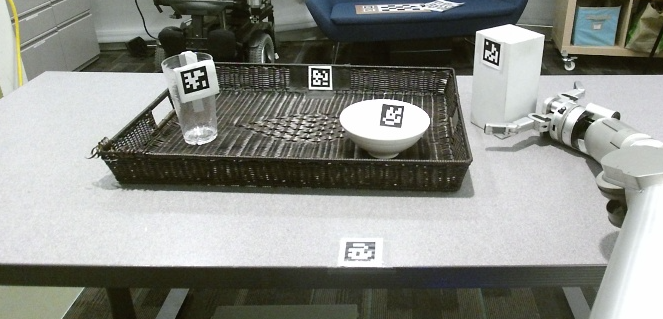
\includegraphics[width=\columnwidth, height=120px]{figs/table_clearing_rgb_small} \\
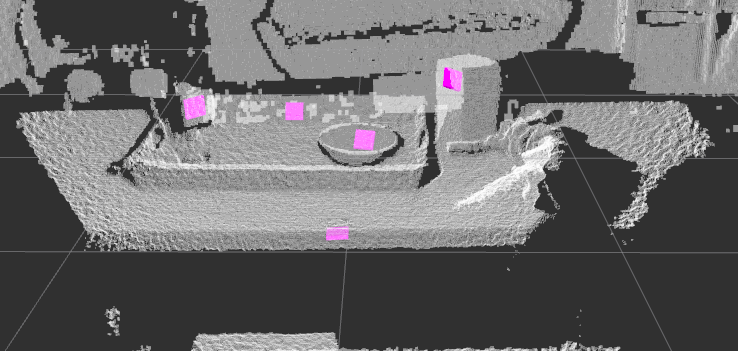
\includegraphics[width=\columnwidth, height=120px]{figs/table_clearing_depth}
\caption{Robot about to execute a manipulation task and rearrange the objects on the table. Apriltags are used to find the poses of targeted objects in the scene but the robot ultimately fails to gasp the rectangular prism because the orientation of its pose is wrong.}
\label{fig:table_clearing}
\end{figure}

\begin{figure}
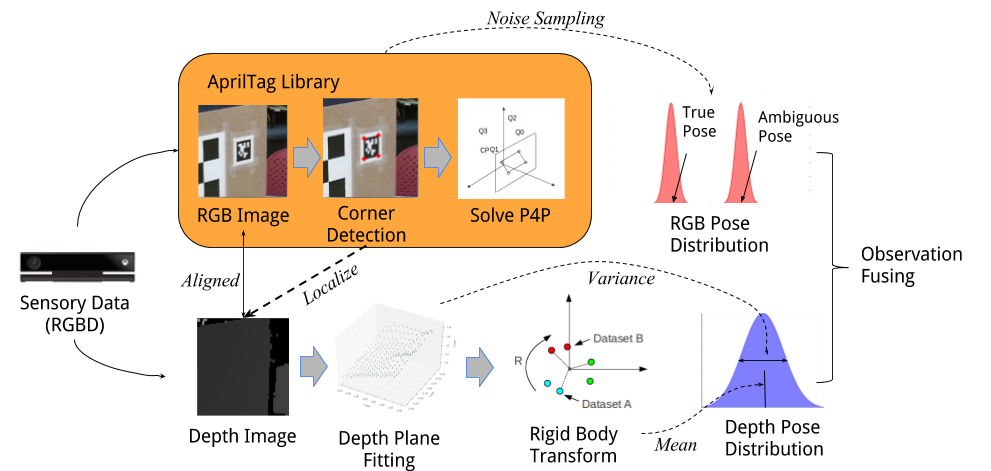
\includegraphics[width=\columnwidth]{figs/pipeline} \\
\caption{An overview of our purposed sensor fusion pipeline. We implicitly generate pose estimations from RGB and depth sensor observations and combine them according to their uncertainty distribution.}
\label{fig:pipeline}
\end{figure}

However, obtaining highly accurate pose estimations using fiducial tags from noisy data remains a challenge. This is  important for robotic applications because small errors can cause large system failures as the errors propagate and amplify through the system as shown in Figure \ref{fig:table_clearing}. Currently, the fiducial tag systems yield promising results under well conditioned or rendered environments, but this does not translate to ill-conditioned settings. For instance, when AprilTags, a state of the art fiducial marker, are used with low resolution cameras or harsh lighting conditions, the system often produces poses with tremendous rotational errors. We observe that the AprilTag's localization accuracy performs significantly worse when there is noise in the captured image. This is a difficult problem because RGB sensors are often sensitive to lighting, and current fiducial systems are not designed to take advantage of other sensors commonly available on robots.

We present two main contributions in this paper. First, we conducted an in-depth analysis on the effect of various noises on the pose estimation process. In particular, the noise in RGB images creates a perspective ambiguity problem that makes the pose estimation challenging without additional information. 

Second, we describe a novel method that takes advantage of the RGBD sensors that are commonly available on most robotic systems to accurately estimate the pose from a single tag under noisy conditions in real time. The overview of our method as shown in Figure \ref{fig:pipeline}. Our key insight is that RGB and depth sensors work optimally in complements. RGB data can be used to efficiently detect features where depth data can retain better structural information. We can leverage this to improve the pose estimation process and increase the localization accuracy under difficult conditions. The key features to this algorithm are: 
\begin{itemize}
\item This method is highly robust to noise in the scene. It can obtain accurate poses suitable for a wide range of robotic applications.   
\item It is easily generalizable to most fiducial tag designs.
\item It has very small computation overhead, and can be ran in real time. 
\end{itemize}

This paper also presents empirical results demonstrating the successful performance of the algorithm on captured data from a humanoid robot. Our implementation of the algorithm is based off of the Apriltag detection pipeline and it is integrated with ROS. 